\documentclass[12pt]{article}

\author{David Gleich}
\title{Matlab BGL v1.0}
\date{23 April 2006}

\usepackage{color}
\definecolor{shadecolor}{rgb}{0.9,0.9,0.9} 
\usepackage{framed}
\usepackage{url}
\usepackage{graphicx}
\usepackage{amsmath}
\usepackage{tabularx}

\usepackage[bf]{caption}

\usepackage{listings}
\lstset{basicstyle={\footnotesize \ttfamily}, columns=flexible,
backgroundcolor=\color{shadecolor},frame=single,
rulesepcolor=\color{black},
xleftmargin=36pt}


\renewcommand{\familydefault}{\sfdefault}
\usepackage{fullpage}
%\setlength{\textheight}{9in}
%\setlength{\topmargin}{-0.5in}
%\setlength{\textwidth}{6.5in}
%\setlength{\oddsidemargin}{0.125in}
%\setlength{\evensidemargin}{0.125in}

\setlength{\parindent}{0in}
\setlength{\parskip}{6pt}

\def\floatpagefraction{.9}      % default .5
\def\topfraction{.9}            % default .7
\def\bottomfraction{.9}         % default .3
\def\textfraction{.1}           % default .2

%\newcommand{\mcode}[1]{\parashade[.95]{roundcorners}{\begin{Verbatim}#1\end{Verbatim}}}
%\newenvironment{mcode}{\begin{lstlisting}}{\end{lstlisting}}
\lstnewenvironment{mcode}{}{}
\lstnewenvironment{mcode-small}{\lstset{basicstyle={\scriptsize \ttfamily}}}{}

\newcommand{\mycmd}[1]{\url{#1}}
\newcommand{\mypath}[1]{{\ttfamily \small #1}}
\DeclareRobustCommand\cs[1]{\texttt{\char`\\#1}} 
\newcommand{\mynote}[1]{\begin{center} \fbox{\hspace{1cm}\bfseries Note: #1\hspace{1cm}}\end{center}}

%\renewcommand{\maketitle}{

\begin{document}

%%% HTML-begin title
{
\setlength{\parskip}{0pt}
\begin{center}
{\Large Matlab BGL v1.0}\\
David Gleich\\
\today
\end{center}
\tableofcontents
%%% HTML-toc
}
%%% HTML-end title

\section{Synopsis}

\begin{mcode}
>> [d ft dt pred] = dfs(A)
>> [d dt pred] = bfs(A);

>> [d pred] = dijkstra_sp(A,u);
>> [d pred] = bellman_ford_sp(A,u);
>> [d pred] = dag_sp(A,u);
>> D = johnson_all_sp(A);
>> D = floyd_warshall_all_sp(A);

>> T = kruskal_mst(A);
>> T = prim_mst(A);

>> cc = components(A)  
>> [a C] = biconnected_components(A);

>> [flow cut R F] = max_flow(A,u,v);
\end{mcode}

\section{Installation}
We are distributing the library as a set of precompiled mex files for Windows and Linux.  Hopefully these work for most people.  In the event that the files do not work, we also distribute a precompiled .lib (Win32) and .a (Linux) file to recompile the mex files for another version of Matlab.  Eventually, we plan to distribute the code behind the .lib and .a files.  

If all goes well, installing the library is as easy as:
\begin{enumerate}
\item	Unzip the file \url{matlab_bgl.zip}.  For the sake of example, let's assume you unzipped it into the same folder as I do: ``\mypath{/home/dgleich/matlab/}'' on Linux and ``\mypath{C:\cs{}Documents and Settings\cs{}dgleich\cs{}My Documents\cs{}matlab\cs{}}'' on Windows.
\item	In Matlab, add either the Linux path ``\mypath{/home/dgleich/matlab/matlab\_bgl/}'' or the Windows path ``\mypath{C:\cs{}Documents and Settings\cs{}dgleich\cs{}My Documents\cs{}matlab\cs{}}'' to the path (but replacing those directories with the ones where you actually unzipped \url{matlab_bgl.zip}).
\end{enumerate}

To test the installation, try running the following script.
\begin{mcode}
% add matlab_bgl to the path
% e.g. addpath('/home/dgleich/matlab/matlab_bgl');
>> clustering_coefficients(sparse(ones(5)))
ans =
     1
     1
     1
     1
     1
\end{mcode}
\subsection*{Building the library}
\mynote{You should not need to complete the following steps!}
In general, the precompiled versions should work.  If they do not and you would like to try compiling the mex files from source, this section explains the process.  On Windows, you must use a Microsoft Visual Studio compiler.  The free Visual Studio 2003 Compiler Toolkit\footnote{\url{http://msdn.microsoft.com/visualc/vctoolkit2003/}} suffices for this purpose.  On Linux, any recent version of gcc should work.

To compile the library from the .lib and .a files, 
\begin{mcode}
>> cd /home/dgleich/matlab/
>> cd matlab_bgl/
>> cd private
>> compile
\end{mcode}
If you cannot compile the library and the example does not work, please send email to \url{mithandor@gmail.com} with as much output as you can.  

\section{Motivation and Implementation}
The Boost Graph Library\footnote{\url{http://www.boost.org/libs/graph/doc/}} is a powerful graph analysis toolkit.  It contains efficient algorithms implemented as generic C++ template specifications.  In the MatlabBGL library, we have wrapped these algorithms with \emph{mex} functions which are callable from Matlab.  The goal of the library was to introduce as little new material in Matlab as possible.  As the next section explains, MatlabBGL uses the Matlab sparse matrix type as the graph type directly.

The idea behind the MatlabBGL library is to provide a rich set of graph-theoretic routines as efficient Matlab functions.  

\subsection{Graphs in Matlab}
Matlab \emph{has} a built in graph type: the sparse matrix.  The goal of the MatlabBGL library is to use the Matlab sparse matrix as a graph type.  To be slightly more concrete, we use a sparse matrix in Matlab to represent the adjacency matrix of two graphs from the Boost Graph library review of graph theory.

\begin{figure}[ht!]
\centering
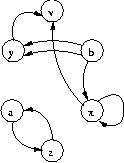
\includegraphics[width=1.5in]{digraph}
\caption{A directed graph.}
\label{fig:digraph}
\end{figure}

For the graph in Figure~\ref{fig:digraph}, the adjacency matrix is 
\[ \begin{pmatrix}
     0  &    0  &   0  &   0  &   0 &    1\\
     0  &   0  &   0   &  1  &   2  &   0\\
     0  &   0  &   0   &  0  &   0  &   0\\
     0  &   0  &   0   &  1  &   0  &   1\\
     0  &   0  &   1   &  0  &   0  &   0\\
     1  &   0  &   0   &  0  &   0  &   0\\
     \end{pmatrix},\]
and we labeled vertex $a=1$, $b=2$, $v=3$, $x=4$, $y=5$, $z=6$.  In the original graph from Figure~\ref{fig:digraph}, there are two edges from $b$ to $y$.  We have replaced both edges with a two in the adjacency matrix.  While this works for many algorithms, there are currently no ways of implemented true multi-graphs in MatlabBGL.

\mynote{There are currently no multi-graphs supported in MatlabBGL.}

We can construct this graph as a Matlab sparse matrix with the following set of commands.

\begin{mcode}
>> A = sparse(6,6);
>> A(1,6) = 1;
>> A(6,1) = 1;
>> A(2,4) = 1;
>> A(2,5) = 2;
>> A(4,4) = 1;
>> A(4,6) = 1;
>> A(5,3) = 1;
>> labels = {'a';'b';'v';'x';'y';'z'};
\end{mcode}

Now, we can use the directed graph as a Matlab sparse matrix and as a MatlabBGL graph.  As we will see, we can treat any square sparse matrix as a MatlabBGL graphs.

\begin{figure}[ht!]
\centering
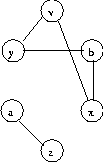
\includegraphics[width=1.5in]{undigraph}
\caption{An undirected graph.}
\label{fig:undigraph}
\end{figure}

MatlabBGL requires that undirected graphs have symmetric adjacency.  When constructing a graph, this means that you must specify each edge twice.  The following Matlab session constructs the graph in Figure~\ref{fig:undigraph}.

\begin{mcode}
>> A = sparse(6,6);
>> A(1,6) = 1;
>> A(6,1) = 1;
>> A(2,4) = 1;
>> A(4,2) = 1;
>> A(2,5) = 1;
>> A(5,2) = 1;
>> A(3,4) = 1;
>> A(4,3) = 1;
>> A(3,5) = 1;
>> A(5,3) = 1;
>> labels = {'a';'b';'v';'x';'y';'z'};
\end{mcode}

An easier way of constructed the graph from Figure~\ref{fig:undigraph} is to take advantage of some of Matlab's sparse matrix routines.  We can use one command to add a reverse edge for each edge listed in a sparse matrix by executing
\begin{mcode}
>> A = max(A,A');
\end{mcode}

Using this command, we can build the undirected graph using the commands:
\begin{mcode}
>> A = sparse(6,6);
>> A(1,6) = 1;
>> A(2,4) = 1;
>> A(5,2) = 1;
>> A(4,3) = 1;
>> A(3,5) = 1;
>> A = max(A,A');
\end{mcode}

In general, any square sparse matrix in Matlab is a MatlabBGL graph; the non-zeros of the matrix define the edges.  If the sparse matrix is symmetric, then the graph is undirected.

\mynote{Any square sparse matrix is a MatlabBGL graph.}




\subsection{Implementation details}
In this section, we will address some fairly technical details of the implementation.  Matlab implements sparse matrices as a set of compressed column arrays.  Most adjacency matrix representations (and the one used in MatlabBGL) use the rows of the matrix to specify the edges from a particular vertex.  That is, $A(i,j) = 1$ indices there is an edge between vertex $i$ and vertex $j$.  

Unfortunately, this means that in the Matlab compressed column storage format, we do not have efficient access to the elements of each row of the matrix (i.e. the adjacent vertices).  The Boost graph algorithms require access to the adjacent vertices.  So, every time we call a MatlabBGL function we transpose the sparse matrix, unless the function requires a symmetric input.

Some algorithms only use the non-zero structure of the sparse matrix.  Other algorithms use the values of the non-zeros as the weights of the edges.  In general, things work the way you expect them to using a sparse adjacency matrix to represent the graph; we have documented any serious deviations from the expected behavior.

Transposing the matrix can be somewhat expensive, so we provide an option to eliminate the transpose \emph{if the user knows better}.  Thus, for the most efficient MatlabBGL runtimes, construct the transpose of the adjacency matrix and run the MatlabBGL routines with the extra option 
\begin{mcode}
>> bfs(A,u,struct('istrans',1));
\end{mcode}

Currently, the \mycmd{max_flow} function performs additional input manipulation and does not have this optimization.  

\section{Examples}
We'll show four examples of how to use the Matlab BGL library.  The first three examples come from the Boost Graph Library samples.  The last example shows how to write a new algorithm using MatlabBGL.

\subsection{Breadth first search}

In the following example, we perform a breadth first search on an example graph from Boost.  This example is implemented in the \mypath{examples/bfs\_example.m} file.

\begin{figure}[ht!]
\centering
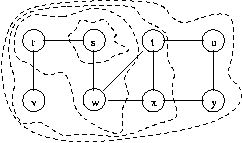
\includegraphics[width=2in]{bfs_example}
\caption{The breadth first search example graph from the Boost Graph Library.  The concentric regions show the order in which breadth first search will visit the vertices.}
\label{fig:bfs}
\end{figure}

We will load the graph from Figure~\ref{fig:bfs} and compute the breadth first search (BFS).

\begin{mcode}
>> load graphs\bfs_example.mat
>> [d dt pred] = bfs(A,2);
>> [ignore order] = sort(dt);
>> labels(order)
ans = 
    's'
    'r'
    'w'
    'v'
    't'
    'x'
    'u'
    'y'
\end{mcode}

The first command loads the graph from the stored representation in Matlab.  As we've seen, we present the graph as a sparse adjacency matrix.  We can look at the full adjacency matrix using the \mycmd{full} command.

\begin{mcode}
>> full(A)
ans =
     0     1     0     0     1     0     0     0     0
     0     0     0     0     1     0     0     0     0
     0     0     0     0     0     1     0     0     0
     0     0     0     0     0     0     0     0     0
     1     0     1     1     0     1     0     0     0
     0     0     0     0     1     0     0     0     0
     0     0     0     0     0     0     0     1     1
     0     0     0     0     0     0     0     0     1
     0     0     0     0     0     0     1     0     0
\end{mcode}

The second command runs the MatlabBGL \mycmd{bfs} command starting from vertex 2.  Looking at the label file, we can see that vertex 2 was really $s$ in the original graph.  The \mycmd{bfs} command returns three vectors: \mycmd{d} is a vector of the distance to each other vertex from $s$; \mycmd{dt} is the discover time of each vertex, the time when the BFS first reached that vertex; and \mycmd{pred} is the predecessor array encoded as a Matlab tree.  In fact, we can view the predecessor array using the \mycmd{treeplot} command.

\begin{mcode}
>> treeplot(pred)
\end{mcode}
\begin{center}
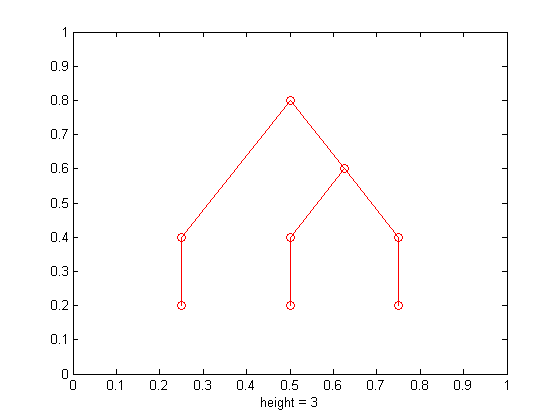
\includegraphics[width=3in]{bfs_treeplot}
\end{center}

The third line of the example sorts the vertices by their discover time and saves the permutation of the indices.  The permutation tells us how to permute the labels array to view the vertex labels in the discover order.  The final line actually prints the labels in their discover order.  Comparing with the original figure, we can see that the vertices were discovered in the correct BFS order.

\subsection{Depth first search}

In this example, we will compute a depth first search (DFS) of the graph in Figure~\ref{fig:dfs}.  This example is implemented in the \mypath{examples/dfs\_example.m} file.

\begin{figure}[ht!]
\centering
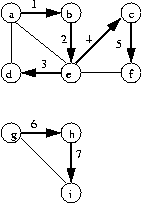
\includegraphics[width=1.25in]{dfs}
\caption{The depth first search example graph from the Boost Graph Library.}
\label{fig:dfs}
\end{figure}

We first load the graph and then call the MatlabBGL \mycmd{dfs} command.  
\begin{mcode}
>> load graphs/dfs_example.mat
>> [d dt ft pred] = dfs(A,1,struct('full',1));
>> [ignore order] = sort(dt);
>> labels(order)
ans = 
    'a'
    'b'
    'e'
    'c'
    'f'
    'd'
    'g'
    'h'
    'i'
\end{mcode}

The \mycmd{dfs} command is similar to the \mycmd{bfs} command.  However, the \mycmd{dfs} routine provides the \mycmd{ft} vector which indicates the finish time for each vertex as well.  The other commands in this script are explained in the first example. 

The graph in Figure~\ref{fig:dfs} is disconnected.  We can use the \mycmd{dfs} command to find all the vertices connected to a source vertex.  

\begin{mcode}
>> load graphs/dfs_example.mat
>> d = dfs(A,1);
>> labels(d < 0)
ans = 
    'g'
    'h'
    'i'
\end{mcode}

This result indicates that nodes $g$, $h$, and $i$ are in a separate component from vertex $a$.  

\subsection{Max-flox min-cut}
The Boost Graph Library provides an implementation of Goldberg's push-relabel maximum flow algorithm.  In this example, we use the \mycmd{max_flow} routine to find the maximum flow of the graph from Figure~\ref{fig:mincut}.  This example is implemented in the \mypath{examples/max\_flow\_example.m} file.  

\begin{figure}[ht!]
\centering
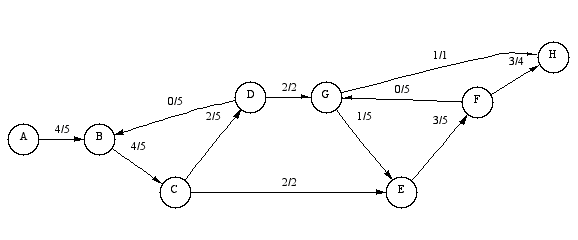
\includegraphics[width=4in]{max-flow}
\caption{The max-flow min-cut example graph from the Boost Graph Library.}
\label{fig:mincut}
\end{figure}

\begin{mcode}
>> load graphs/max_flow_example.mat
>> max_flow(A,1,8)
ans =
     4
>> [flow cut R F] = max_flow(A,1,8);
>> full(R)     
ans =
     0     1     0     0     0     0     0     0
     0     0     1     0     0     0     0     0
     0     0     0     3     0     0     0     0
     0     5     0     0     0     0     0     0
     0     0     0     0     0     2     0     0
     0     0     0     0     0     0     5     1
     0     0     0     0     4     0     0     0
     0     0     0     0     0     0     0     0
\end{mcode}

The script presents two results from the \mycmd{max_flow} routine.  The first call computes the maximum flow from $A$ to $H$.  The second call prints the residual flow graph $R$.  In comparison with Figure~\ref{fig:mincut}, the residual shows the unused capacity on each edge. On the edge from $A$ to $B$, there is only one unit of unused flow, so $R(1,2) = 1$.  

\subsection{New algorithms}
In this section, we will implement a new algorithm using the core set of routines provided by the MatlabBGL library.

\paragraph{Multiway Cut}

The Matlab code for this example is in the file \mypath{examples/multiway\_example.m}.  
Given an undirected graph $G=(V,E)$ with weighted edges $w$.  The multiway cut problem is to find a minimum cost set of edges, $C$, to remove that will disconnect a subset of vertices $S$ from each other.  That is, after we remove the edges $C$ from $G$, there is no path from any vertex $s \in S$ to any other vertex in $S$.  

This problem is NP-complete, but we can find a 2-approximation by solving $|S|$ separate max-flow subproblems.\footnote{Approximation Algorithms.  Vijay V. Vazirani.}  Label the vertices in $S$, $s_1, s_2, \ldots, s_k$, so $k = |S|$.  In each max-flow subproblem, we pick vertex $s_i \in S$ and add a new vertex $t$.  For each $s_j, j\not=i$, we add a directed edge of infinite capacity from $s_j$ to $t$.  We solve the max-flow problem and add the set of edges in the induced min-cut to the set $C$.  

The MatlabBGL implementation of this algorithm follows.

\begin{mcode}
function C = approx_multiway_cut(A,vs)
function C = approx_multiway_cut(A,vs)
% APPROX_MULTIWAY_CUT Solve a 2-approximation to the multi-way cut problem
% 
% C = approx_multiway_cut(A,vs)
%
% Outputs C, the set of edges cut in a 2-approximation to the multiway cut
% problem.  The multiway-cut problem is to find a minimum cost set of edges
% to disconnect all the vertices in vs from each other.
%
% The non-zero values contain the weight of each edge.
%
% The input A must be a symmetric graph.

if (~isequal(A,A'))
    error('approx_multiway_cut:invalidParameter',...
        'the matrix must be symmetric.');
end;

if (min(min(A)) < 0)
    error('approx_multiway_cut:invalidParameter',...
        'the matrix cannot contain negative weights.');
end;

n = size(A,1);

% this should be larger than any conceivable flow...
int_infinity = sum(sum(A))+2*sum(sum(A(vs,:)))+1;

% initial the cut to nothing.
C = sparse(n,n);

% Get A as an edge list...
[i j v] = find(A);

for (kk=1:length(vs))
    v = vs(kk);
    others = setdiff(vs,v);
    
    % Each flow problem add a fake sink as the n+1 vertex
    Aflow = A;
    Aflow(others,n+1) = int_infinity*ones(length(others),1);
    Aflow(n+1,:) = sparse(n+1,1);
    
    % solve the max-flow problem
    [flow ci] = max_flow(Aflow,v,n+1);
    
    % remove the last (fake) entry from the cut.
    ci = ci(1:end-1);
    
    % construct a value over the edges that is 0 except on the cut, we know
    % all values are positive, so just take the absolute value
    vc = abs(v.*(ci(i)-ci(j)))./2;
    
    % add the set of edges to the cut by constructing a sparse matrix with
    % only the cut edges.
    C = C+ sparse(i, j, vc, n,n);
end;
\end{mcode}

We can use this new algorithm to find a set of roads to remove to disconnect a set of nodes.  The following example loads the road network for Minnesota and chooses a set of 125 vertices, calls the \mycmd{approx_multiway_cut} command above, and then draws the cut using the \mycmd{gplot} command.  

\begin{mcode}
load graphs/minnesota.mat

n = size(A,1);
k1 = 75;
k2 = 50;
start1 = 1;
start2 = 800;
vs1 = start1:start1+k1;
vs2 = start2:start2+k2;
vs = [vs1 vs2];
C = approx_multiway_cut(A,vs);

gplot(triu(A),xy,':');
hold on;
gplot(triu(C),xy,'r-');
plot(xy(vs,1),xy(vs,2),'.');
hold off;
set(gca,'XTick',[]);
set(gca,'YTick',[]);
\end{mcode}

When drawing the graphs, we use the \mycmd{triu} command to only select the upper triangular portion of the adjacency matrix.  Otherwise, Matlab will draw both edges, instead of only one edge.  The figure produced by this program follows.

\begin{center}
\includegraphics[width=3in]{multiway_cut-crop}
\end{center}

\section{Features not implemented}

This section contains a list of features that I think should be in MatlabBGL and are currently missing.  If you agree, please send me an email.

\begin{itemize}
\item max-flow intermediate data: Currently, the max-flow algorithm generates a large amount of intermediate data that could be cached between calls if the underlying graph does not change.  
\item support for more algorithms from the Boost Graph Library: I chose not to implement more algorithms from Boost until there is demand or time allows.  The matrix ordering commands are redundant in Matlab because they are already built in.
\item edge labeled graph type: The support for graphs with edge labels is limited.  Although the Matlab sparse matrix type easily supports subgraphs, for a graph with edge labels, computing a subgraph is more difficult.  
\item better graph drawing tools.
\end{itemize}



\section{Reference}

\subsection{Sample Graphs}
This section lists the set of sample graphs provided with MatlabBGL.  The table should be read as \mycmd{clr-26-1.mat} is a directed, weighted graph without labels or node coordinates, the graph came from CLR Figure 26-1.  The source CLR is   The source KT is Kleinberg and Tardos, Algorithm Design.  
\begin{center}
\begin{tabularx}{\linewidth}{c|cc|cc|X}
\textbf{Name} & \textbf{Dir.} & \textbf{Weighted} & \textbf{Labels} & \textbf{Coords.} & \textbf{Source}\\
\hline
clr-24-1 & & $\times$ & $\times$ & $\times$ & CLR\footnote{Corman, Leiserson, and Rivest. Introduction
 to Algorithms, 2nd Edition.} Fig. 24.1\\
clr-25-2 & $\times$ & $\times$ & $\times$ & & CLR Fig. 25.2\\
clr-26-1 & $\times$ & $\times$ & & & CLR Fig. 26.1\\
clr-27-1 &  $\times$ & $\times$ & & & CLR Fig. 27.1\\
kt-3-2 &  &  & & & KT\footnote{ Kleinberg and Tardos. Algorithm Design} Fig. 3.2\\
kt-3-7 & $\times$ &  & & & KT Fig. 3.7\\
kt-6-23 & $\times$ & $\times$ & $\times$ & & KT Fig. 6.23\\
kt-7-2 & $\times$ & $\times$ & $\times$& & KT Fig. 7.2\\
tarjan-biconn & & & & $\times$ & Tarjan\footnote{Tarjan.  Depth-first search and linear graph algorithms, 1972.} Fig. 2\\
padgett-florentine & & & $\times$ & $\times$ &  Website\footnote{\url{http://mrvar.fdv.uni-lj.si/sola/info4/uvod/part4.pdf}}\\
minnesota & & & $\times$ & $\times$ & Highway Data\footnote{National Highway Planning Network, 2003.}\\
tapir & & & & $\times$ & meshpart\footnote{Gilbert and Teng, meshpart toolkit.} \\
cs-stanford & $\times$ & & $\times$ & & Partial webbase 2001 crawl\footnote{Accessed via \url{http://law.dsi.unimi.it/index.php?option=com_include&Itemid=65}.}
\end{tabularx}
\end{center}

\newpage
\hrule
\subsection*{Searches}
\vspace{1cm}
\hrule
\subsubsection*{bfs}
\begin{mcode}
  BFS Compute the breadth first search order.
 
  [d dt pred] = bfs(A,u) returns the distance to each vertex (d) and the  
  discover time (dt) in a breadth first search starting from vertex u.
     d(i) = dt(i) = -1 if vertex i is not reachable from vertex u.
  pred is the predecessor array.  pred(i) = 0 if vertex (i)  
  is in a component not reachable from u and i != u.
 
  This method works on directed graphs.
  The runtime is O(V+E).
 
  ... = bfs(A,u,options) sets optional parameters (see 
  set_matlab_bgl_options) for the standard options.
    There are no additional options for this function.
 
  Note: this function does not depend upon the non-zero values of A, but
  only uses the non-zero structure of A.
 
  Example:
     load graphs/bfs_example.mat
     d = bfs(A,1)
 
  See also DFS
\end{mcode}
\newpage
\subsubsection*{dfs}
\begin{mcode}
  DFS Compute the depth first search times.
 
  [d dt ft pred] = dfs(A,u) returns the distance (d), the discover (dt) and
  finish time (ft) for each vertex in the graph in a depth first search 
  starting from vertex u.
    d = dt(i) = ft(i) = -1 if vertex i is not reachable from u
  pred is the predecessor array.  pred(i) = 0 if vertex (i)  
  is in a component not reachable from u and i != u.
  
  ... = dfs(A,u,options) sets optional parameters (see 
  set_matlab_bgl_options) for the standard options.
    options.full: compute the full dfs instead of the dfs of
       the current component (see Note 1) [{0} | 1]
 
  Note 1: When computing the full dfs, the vertex u is ignored, vertex 1 is
  always used as the starting vertex.  
 
  Note: this function does not depend upon the non-zero values of A, but
  only uses the non-zero structure of A.
 
  Example:
     load graphs/dfs_example.mat
     d = dfs(A,1)
 
  See also BFS
\end{mcode}
\newpage
\hrule
\subsection*{Components}
\vspace{1cm}
\hrule
\subsubsection*{components}
\begin{mcode}
  COMPONENTS Compute the connected components of a graph.
 
  [ci sizes] = components(A) returns the component index vector (ci) and
  the size of each of the connected components (sizes).  The number of
  connected components is max(components(A)).  The algorithm used computes
  the strongly connected components of A, which are the connected
  components of A if A is undirected (i.e. symmetric).  
 
  This method works on directed graphs.
  The runtime is O(V+E), the algorithm is just depth first search.
 
  ... = components(A,u,options) sets optional parameters (see 
  set_matlab_bgl_options) for the standard options.
    There are no additional options for this function.
 
  Note: this function does not depend upon the non-zero values of A, but
  only uses the non-zero structure of A.
 
  Example: 
     load graphs/dfs_example.mat
     components(A)
 
  See also DMPERM, BICONNECTED_COMPONENTS
\end{mcode}
\newpage
\subsubsection*{biconnected\_components}
\begin{mcode}
  BICONNECTED_COMPONENTS Compute the biconnected components and
  articulation points for a symmetric graph A.
 
  [a C] = biconnected_components(A) returns a list of articulation points 
  a and the component graph C where each non-zero indicates the connected
  component of the edge.  That is, C is a matrix with the same non-zero
  structure as A, but with the values replaced with the index of the
  biconnected component of that edge.  The vector a is a list of
  articulation points in the graph.  Articulation points are vertices that
  belong to more than one biconnected component.  Removing an articulation
  point disconnects the graph.
 
  If C is not requested, it is not built.
 
  This method works on undirected graphs.
  The runtime is O(V+E), the algorithm is just depth first search.
 
  ... = biconnected_components(A,optionsu) sets optional parameters (see 
  set_matlab_bgl_options) for the standard options.
    There are no additional options for this function.
 
  Note: the input to this function must be symmetric, so this function
  ignores the 'notrans' default option and never transposes the input.
 
  Note: this function does not depend upon the non-zero values of A, but
  only uses the non-zero structure of A.
 
  Example:
     load graphs/tarjan-biconn.mat
     biconnected_components(A)
 
  See also COMPONENTS
\end{mcode}
\newpage
\hrule
\subsection*{Shortest Paths}
\vspace{1cm}
\hrule
\subsubsection*{shortest\_paths}
\begin{mcode}
  SHORTEST_PATHS Compute the weighted single source shortest path problem.
 
  [d pred] = shortest_paths(A,u) returns the distance (d) and the predecessor
  (pred) for each of the vertices along the shortest path from u to every
  other vertex in the graph.  
  
  ... = shortest_paths(A,u,options) sets optional parameters (see 
  set_matlab_bgl_options) for the standard options.
    options.algname: the algorithm to use 
        [{'auto'} | 'dijkstra' | 'bellman_ford' | 'dag']
    options.inf: the value to use for unreachable vertices 
        [double > 0 | {Inf}]
 
  Note: 'auto' cannot be used with 'nocheck' = 1.  The 'auto' algorithm
  checks if the graph has negative edges and uses bellman_ford in that
  case, otherwise, it uses 'dijkstra'.  In the future, it may check if the
  graph is a dag and use 'dag'.  
 
  Example:
     load graphs/clr-25-2.mat
     shortest_paths(A,1)
     shortest_paths(A,1,struct('algname','bellman_ford'))
 
  See also DIJKSTRA_SP, BELLMAN_FORD_SP, DAG_SP
\end{mcode}
\newpage
\subsubsection*{all\_shortest\_paths}
\begin{mcode}
  all_shortest_paths Compute the weighted all pairs shortest path problem.
 
  D = all_shortest_paths(A) returns the distance matrix D for all vertices
  where D(i,j) indicates the shortest path distance between vertex i and
  vertex j.  
  
  ... = all_shortest_paths(A,u,options) sets optional parameters (see 
  set_matlab_bgl_options) for the standard options.
    options.algname:: the algorithm to use 
        [{'auto'} | 'johnson' | 'floyd_warshall']
    options.inf: the value to use for unreachable vertices 
        [double > 0 | {Inf}]
 
  Note: 'auto' cannot be used with 'nocheck' = 1.  The 'auto' algorithms
  checks the number of edges in A and if the graph is more than 10% dense,
  it uses the Floyd-Warshall algorithm instead of Johnson's algorithm.
 
  Example:
     load graphs/clr-26-1.mat
     floyd_warshall_all_sp(A)
 
  See also JOHNSON_ALL_SP, FLOYD_WARSHALL_ALL_SP.
\end{mcode}
\newpage
\subsubsection*{dijkstra\_sp}
\begin{mcode}
  DIJKSTRA_SP Compute the weighted single source shortest path problem.
 
  Dijkstra's algorithm for the single source shortest path problem only
  works on graphs without negative edge weights.
 
  This method works on weighted directed graphs without negative edge
  weights.
  The runtime is O(V log (V)).
 
  See the shortest_paths function for calling information.  This function 
  just calls shortest_paths(...,struct('algname','dijkstra'));
 
  Example:
     load graphs/clr-25-2.mat
     dijkstra_sp(A,1)
 
  See also SHORTEST_PATHS, BELLMAN_FORD_SP.
\end{mcode}
\newpage
\subsubsection*{bellman\_ford\_sp}
\begin{mcode}
  BELLMAN_FORD_SP Compute the weighted single source shortest path problem.
 
  The Bellman-Ford algorithm for the single source shortest path problem
  works on graphs with negative edge weights.  
 
  See the shortest_paths function for calling information.  This function 
  just calls shortest_paths(...,struct('algname','bellman_ford'));
 
  This method works on weighted directed graphs with negative edge weights.
  The runtime is O(VE).
 
  Example:
     load graphs/kt-6-23.mat
     d = bellman_ford_sp(A,1);
 
  See also SHORTEST_PATHS, DIJKSTRA_SP.
\end{mcode}
\newpage
\subsubsection*{dag\_sp}
\begin{mcode}
  DAG_SP Compute the weighted single source shortest path problem.
 
  The DAG shortest path algorithm for the single source shortest path
  problem only works on directed acyclic-graphs (DAGs).  
 
  If the graph is not a DAG, the results are undefined.  In the future, the
  function may throw an error if the graph is not a DAG.
 
  See the shortest_paths function for calling information.  This function 
  just calls shortest_paths(...,struct('algname','dag'));
 
  This algorithm works on weighted directed acyclic graphs.
  The runtime is O(V+E)
 
  ... = clustering_coefficients(A,options) sets optional parameters (see 
  set_matlab_bgl_options) for the standard options.
     There are no additional options for this function.
 
  Example:
     load graphs/kt-3-7.mat
     dag_sp(A,1)
 
  See also SHORTEST_PATHS
\end{mcode}
\newpage
\subsubsection*{johnson\_all\_sp}
\begin{mcode}
  JOHNSON_ALL_SP Compute the weighted all-pairs shortest path problem.
 
  Johnson's algorithm for the all-pairs shortest path problem 
  works only on graphs without negative edge weights.  This method should
  be used over the Floyd-Warshall algorithm for sparse graphs.  
 
  This method works on weighted directed graphs.
  The runtime is O(VE log(V)).
 
  See the shortest_paths function for calling information.  This function 
  just calls all_shortest_paths(...,struct('algname','johnson'));
 
  Example:
     load graphs/clr-26-1.mat
     floyd_warshall_all_sp(A)
 
  See also ALL_SHORTEST_PATHS, FLOYD_WARSHALL_ALL_SP.
\end{mcode}
\newpage
\subsubsection*{floyd\_warshall\_all\_sp}
\begin{mcode}
  FLOYD_WARSHALL_ALL_SP Compute the weighted all-pairs shortest path problem.
 
  The Floyd-Warshall algorithm for the all-pairs shortest path problem 
  works only on graphs without negative edge weights.  This method should
  be used over the Johnson algorithm for dense graphs.  
 
  This method works on weighted directed graphs.
  The runtime is O(V^3).
 
  See the shortest_paths function for calling information.  This function 
  just calls all_shortest_paths(...,struct('algname','floyd_warshall'));
 
  Example:
     load graphs/clr-26-1.mat
     floyd_warshall_all_sp(A)
 
  See also ALL_SHORTEST_PATHS, JOHNSON_ALL_SP.
\end{mcode}
\newpage
\hrule
\subsection*{Minimum Spanning Trees}
\vspace{1cm}
\hrule
\subsubsection*{mst}
\begin{mcode}
  MST Compute a minimum spanning tree for an undirected graph A.
 
  There are two ways to call MST.
  T = mst(A)
  [i j v] = mst(A) 
  The first call returns the minimum spanning tree T of A.  
  The second call returns the set of edges in the minimum spanning tree.  
  The calls are related by 
     T = sparse(i,j,v,size(A,1), size(A,1)); 
     T = max(T,T');
  The optional algname parameter chooses which algorithm to use to compute
  the minium spanning tree.  Note that the set of edges returned is not
  symmetric and the final graph must be explicitly symmetrized.
 
  This method works on undirected graphs graphs.
 
  ... = mst(A,optionsu) sets optional parameters (see 
  set_matlab_bgl_options) for the standard options.
    options.algname: the minimum spanning tree algorithm
      [{'prim'} | 'kruskal']
 
  Note: the input to this function must be symmetric, so this function
  ignores the 'notrans' default option and never transposes the input.
 
  Example:
     load graphs/clr-24-1.mat
     mst(A)
 
  See also PRIM_MST, KRUSKAL_MST
\end{mcode}
\newpage
\subsubsection*{kruskal\_mst}
\begin{mcode}
  KRUSKAL_MST Compute a minimum spanning with Kruskal's algorithm.
 
  The Kruskal MST algorithm computes a minimum spanning tree for a graph.
 
  This method works on weighted symmetric graphs.
  The runtime is O(E log (E)).
 
  See the mst function for calling information.  This function just calls
  mst(...,struct('algname','kruskal'));
 
  Example:
     load graphs/clr-24-1.mat
     kruskal_mst(A)
 
  See also MST, PRIM_MST.
\end{mcode}
\newpage
\subsubsection*{prim\_mst}
\begin{mcode}
  PRIM_MST Compute a minimum spanning with Kruskal's algorithm.
 
  Prim's MST algorithm computes a minimum spanning tree for a graph.
 
  This method works on weighted symmetric graphs without negative edge
  weights.
  The runtime is O(E log (V)).
 
  See MST for calling information.  This function just calls
  mst(...,struct('algname','prim'));
 
  Example:
     load graphs/clr-24-1.mat
     prim_mst(A)
 
  See also MST, KRUSKAL_MST.
\end{mcode}
\newpage
\hrule
\subsection*{Statistics}
\vspace{1cm}
\hrule
\subsubsection*{clustering\_coefficients}
\begin{mcode}
  CLUSTERING_COEFFICIENTS Compute the clustering coefficients for vertices.
 
  ccfs = clustering_coefficients(A) returns the clustering coefficients for
  all vertices in A.  The clustering coefficient is the ratio of the number
  of edges between a vertex's neighbors to the total possible number of 
  edges between the vertex's neighbors. 
 
  This method works on directed or undirected graphs.
  The runtime is O(nd^2) where d is the maximum vertex degree.
 
  ... = clustering_coefficients(A,options) sets optional parameters (see 
  set_matlab_bgl_options) for the standard options.
    There are no additional options for this function.
 
  Note: this function does not depend upon the non-zero values of A, but
  only uses the non-zero structure of A.
 
  Example:
     load graphs\clique-10.mat
     clustering_coefficients(A)
\end{mcode}
\newpage
\subsubsection*{betweenness\_centrality}
\begin{mcode}
  BETWEENNESS_CENTRALITY Compute the betweenness centrality for vertices.
 
  bc = betweenness_centrality(A) returns the betweenness centrality for
  all vertices in A.  
 
  This method works on weighted or weighted directed graphs.
  For unweighted graphs (options.unweighted=1), the runtime is O(VE).
  For weighted graphs, the runtime is O(VE + V(V+E)log(V)).
 
  ... = betweenness_centrality(A,options) sets optional parameters (see 
  set_matlab_bgl_options) for the standard options.
    options.unweighted: use the slightly more efficient unweighted
      algorithm in the case where all edge-weights are equal [{0} | 1]  
 
  Example:
     load graphs/padgett-florentine.mat
     betweenness_centrality(A)
\end{mcode}
\newpage
\hrule
\subsection*{Flow}
\vspace{1cm}
\hrule
\subsubsection*{max\_flow}
\begin{mcode}
  MAX_FLOW Compute the max flow on A from u to v.
 
  flowval=max_flow(A,u,v) computes the maximum flow on the network defined by
  the adjacency structure A, with source u and sink v.
 
  [flowval cut R F] = max_flow(A,u,v) returns the maximum flow in the 
  network A with source u and sink v as well as additional information.  
  For each vertex on the source side of the mincut, mincut(i) = 1, 
  for each vertex on the sink side, mincut(i) = -1.  
  R is the residual graph.  R(i,j) is the amount of unused capacity 
  on edge (i,j).  F is the flow graph, F(i,j) is the amount of used 
  capacity on edge (i,j).  F, A, and R satisfy the relationship A = F + R.
 
  The algorithm used is the push-relabel algorithm.
 
  ... = max_flow(A,optionsu) sets optional parameters (see 
  set_matlab_bgl_options) for the standard options.
    There are no additional options for this function.
 
  Note: the values on A are interpreted as integers, please round them
  yourself to get the best interpretation.  The code uses the floor of 
  the values in A.
 
  Example:
     load graphs\max_flow_example.mat
     max_flow(A,1,8)
\end{mcode}

\end{document}